\documentclass[10pt,a4paper]{article}
\usepackage[utf8]{inputenc}
\usepackage[russian]{babel}
\usepackage{amsmath}
\usepackage{amsfonts}
\usepackage{amssymb}
\usepackage{graphicx}
\author{Агафонова Оксана}
\title{LaTeX}
\begin{document}
\maketitle
\clearpage
\tableofcontents
\clearpage
\section{Cистема верстки \TeX{} и расширения \LaTeX{}}

\subsection{Цель работы}

\hspace{0,6cm}Изучение принципов верстки \TeX{}, создание первого отчёта.

\subsection{Ход работы}

\hspace{0,6cm}\LaTeX{} --- наиболее популярный набор макрорасширений (или макропакет) системы компьютерной вёрстки \TeX{}, который облегчает набор сложных документов. 

Общий внешний вид документа в LaTeX определяется стилевым файлом. Существует несколько стандартных стилевых файлов для статей, книг, писем и т. д., кроме того, многие издательства и журналы предоставляют свои собственные стилевые файлы, что позволяет быстро оформить публикацию, соответствующую стандартам издания.

Во многих развитых компьютерных аналитических системах, например, Maple, Mathematica, Maxima, Reduce возможен экспорт документов в формат *.tex. Для представления формул в Википедии также используется TeX-нотация.

Термин LaTeX относится только к языку разметки, он не является текстовым редактором. Для того, чтобы создать документ с его помощью, надо набрать .tex-файл с помощью какого-нибудь текстового редактора. В принципе, подойдёт любой редактор, но большая часть людей предпочитает использовать специализированные, которые так или иначе облегчают работу по набору текста LaTeX-разметки.

Будучи распространяемым под лицензией LaTeX Project Public License, LaTeX относится к свободному программному обеспечению.

\subsubsection{Система набора}
\hspace{0,6cm}Главная идея \LaTeX{} состоит в том, что авторы должны думать о содержании, о том, что они пишут, не беспокоясь о конечном визуальном облике (печатный вариант, текст на экране монитора или что-то другое). Готовя свой документ, автор указывает логическую структуру текста (разбивая его на главы, разделы, таблицы, изображения), а LaTeX решает вопросы его отображения. Так содержание отделяется от оформления. Оформление при этом или определяется заранее (стандартное), или разрабатывается для конкретного документа.

Это похоже на стили оформления, которые используются в текстовых процессорах, или на использование стилевых таблиц в HTML.

\subsubsection{Возможности}
\hspace{0,6cm}Возможности системы, в принципе, не ограничены (из-за механизма программирования новых макросов). Вот список некоторых возможностей, предлагаемых стандартными макросами и теми, которые можно скачать  с сервера CTAN:
\begin{itemize}
\item алгоритмы расстановки переносов, определения междусловных пробелов, балансировки текста в абзацах;
\item автоматическая генерация содержания, списка иллюстраций, таблиц и т. д.;
механизм работы с перекрёстными ссылками на формулы, таблицы, иллюстрации, их номер или страницу;
\item механизм цитирования библиографических источников, работы с библиографическими картотеками;
\item размещение иллюстраций (иллюстрации, таблицы и подписи к ним автоматически размещаются на странице и нумеруются);
\item оформление математических формул, возможность набирать многострочные формулы, большой выбор математических символов;
\item оформление химических формул и структурных схем молекул органической и неорганической химии;
\item оформление графов, схем, диаграмм, синтаксических графов;
\item оформление алгоритмов, исходных текстов программ (которые могут включаться в текст непосредственно из своих файлов) с синтаксической подсветкой;
\item разбивка документа на отдельные части (тематические карты).
\end{itemize}

\subsubsection{Оболочка TexMaker}

\hspace{0,6cm}Texmaker является мощным редактором текста и исходного кода, работающий с языком разметки LaTeX. Он позволяет форматировать текст и готовить многостраничные документы к печати. Редактор предоставляет возможность работы с библиографическими списками, оглавлением и другими атрибутами профессионального оформления. В Texmaker есть так же возможность конвертирования документов в различные форматы, функции сворачивания блоков кода и автозавершения кода, встроенный просмотрщик PDF документов и многое другое. Внешний вид редактора представлен на рисунке 1.

\begin{figure}[h!]
\centering
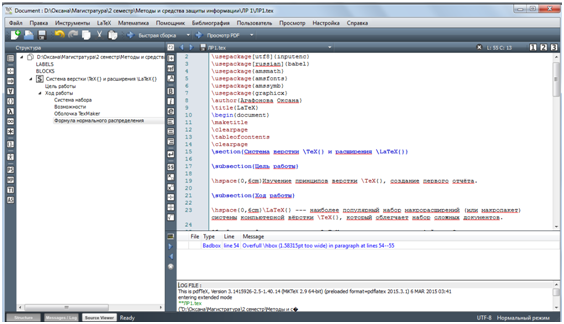
\includegraphics[scale=0.65]{res/TexMaker}
\caption{Редактор TexMaker}
\end{figure}

\subsubsection{Формула нормального распределения}
\hspace{0,6cm}Нормальное распределение, также называемое распределением Гаусса — распределение вероятностей, которое в одномерном случае задается функцией плотности вероятности, совпадающей с функцией Гаусса:
\begin{equation}
\frac{1}{\sigma\sqrt{2\pi}}
   \exp\left(-\frac{(x-\mu)^2}{2\sigma^2}\right)
\end{equation}

\subsection{Выводы}

\hspace{0,6cm}\LaTeX{} наиболее популярный набор макрорасширений (или макропакет) системы компьютерной вёрстки \TeX{}, который облегчает набор сложных документов.

Пакет позволяет автоматизировать многие задачи набора текста и подготовки статей, включая набор текста на нескольких языках, нумерацию разделов и формул, перекрёстные ссылки, размещение иллюстраций и таблиц на странице, ведение библиографии и др. Кроме базового набора существует множество пакетов расширения \LaTeX{}.

\newpage
\section{Система контроля версий Git}

\subsection{Цель работы}
Изучить систему контроля версий Git, освоить основные приёмы работы с ней.

\subsection{Ход работы}

\begin{itemize}

\item{Получить содержимое репозитория
\begin{verbatim}git clone https://github.com/OksanaAgafonova/InfoSecCourse2015.git
\end{verbatim}}

\item{Добавить новую папку и первого файла под контроль версий
\begin{verbatim}cd InfoSecCourse2015/
mkdir folder
cd folder
echo 1 >> file
git add --all
\end{verbatim}}

\item{Зафиксировать изменения в локальном репозитории
\begin{verbatim}git commit -a -m "file add"
\end{verbatim}}

\item{Внести изменения в файл и просмотреть различия
\begin{verbatim}echo 2 >> file
git diff master:./file ./file
\end{verbatim}}

\item{Отменить локальные изменения
\begin{verbatim}git reset HEAD ./file
git checkout ./file
\end{verbatim}}

\item{Внести изменения в файл и просмотреть различия
\begin{verbatim}echo 3 >> file
git diff master:./file ./file
\end{verbatim}}

\item{Зафиксировать изменения в локальном репозитории, зафиксировать изменения в центральном репозитории
\begin{verbatim}git commit -a -m "file changed"
git push
\end{verbatim}}

\item{Получить изменения из центрального репозитория
\begin{verbatim}git pull
\end{verbatim}}

\end{itemize}

\subsection{Выводы}

\hspace{0,6cm}Git --- распределённая система управления версиями файлов. Проект был создан Линусом Торвальдсом для управления разработкой ядра Linux, первая версия выпущена 7 апреля 2005 года. На сегодняшний день его поддерживает Джунио Хамано.

\newpage
\section{Cоздание электронных цифровых подписей c PGP}

\subsection{Цель работы}
\hspace{0,6cm}Научиться создавать сертификаты, шифровать файлы и ставить ЭЦП.

\subsection{Ход работы}

\subsubsection{Знакомство с пакетом Kleopatra}

\hspace{0,6cm}Kleopatra это графический интерфейс к GnuPG и предназначенных для работы под окружением KDE и портированный на MS Windows (доступные в составе пакета Gpg4win). Внешний вид пакета представлен на рисунке 2.

\begin{figure}[h!]
\centering
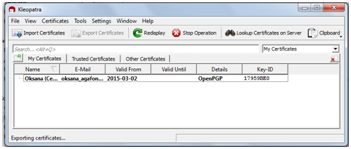
\includegraphics[scale=0.67]{res/Kleopatra}
\caption{Графический интерфейс Kleopatra}
\end{figure}

\hspace{0,6cm} Произведен экспорт сертификата в файл с расширением .asc

\begin{figure}[h!]
\centering
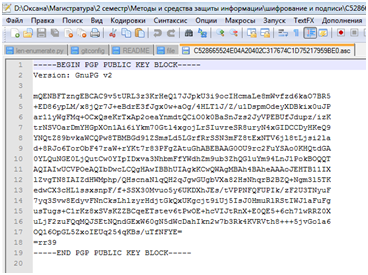
\includegraphics[scale=0.67]{res/Sertifikat}
\caption{Сертификат в формате asc}
\end{figure}

\hspace{0,6cm}Импортирован чужой сертификат (см.рис.4)

\begin{figure}[h!]
\centering
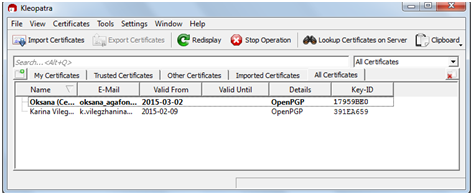
\includegraphics[scale=0.67]{res/Sertifikat2}
\caption{Импорт чужого сертификата}
\end{figure}

\hspace{0,6cm} Попыталась расшифровать ваш файл karina.asc, не получилось, вышло следующее сообщение(см.рис.5):

\begin{figure}[h!]
\centering
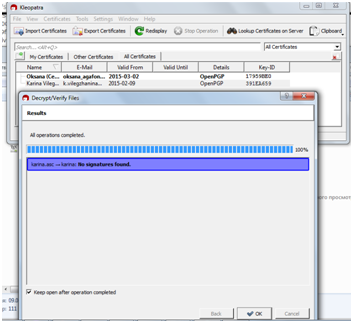
\includegraphics[scale=0.67]{res/Rasshifr}
\caption{Расшифровка файла karina.asc}
\end{figure}

\end{document}